\documentclass[12pt]{article}
\usepackage[margin=1in]{geometry}
\usepackage{graphicx}
\graphicspath{ {./} }


\title{Talkatiel Software Requirements and Planning}
\author{Brendan Byers, Ryan Sisco, Iliana J, Aidan Grimshaw}
\date{\today}

\begin{document}
\begin{center}
      \Large\textbf{Talkatiel Software Design Specification and User Interface}\\
      \large\textit{Brendan Byers, Ryan Sisco, Iliana Javier, Aidan Grimshaw, Yufei Zeng}\\
      \large{byersbr, siscor, javieri, grimshaa, zengyu}\\
   \end{center}

\tableofcontents

\section{User Interface Prototypes}
We have created three user interface prototypes to showcase the key user interactions that will make our app functional.

<<<<<<< HEAD
\subsection{User Interface Elements}
\begin{center}
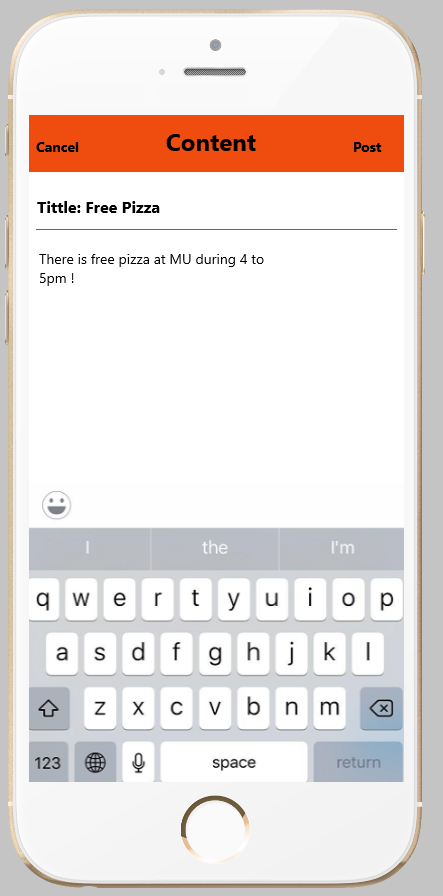
\includegraphics[scale=0.30]{img/ui/post}\linebreak
\textbf{Creating a New Post UI}
  \end{center}

\subsection{Creating a New Post}
Users create a new post with a title and text content. When they press the submit button, a new post element is added to the database, with the attributes of title, text content, submission time, upvote/downvote count, and author as specified by the post class diagram.
\begin{center}
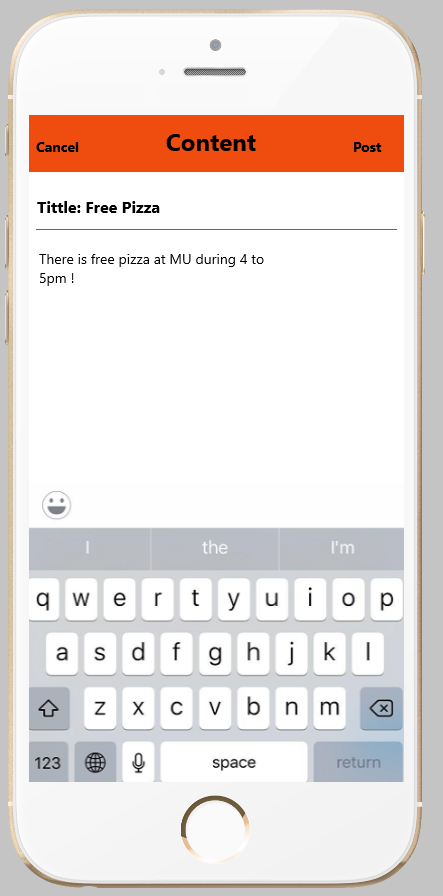
\includegraphics[scale=0.30]{img/ui/post}
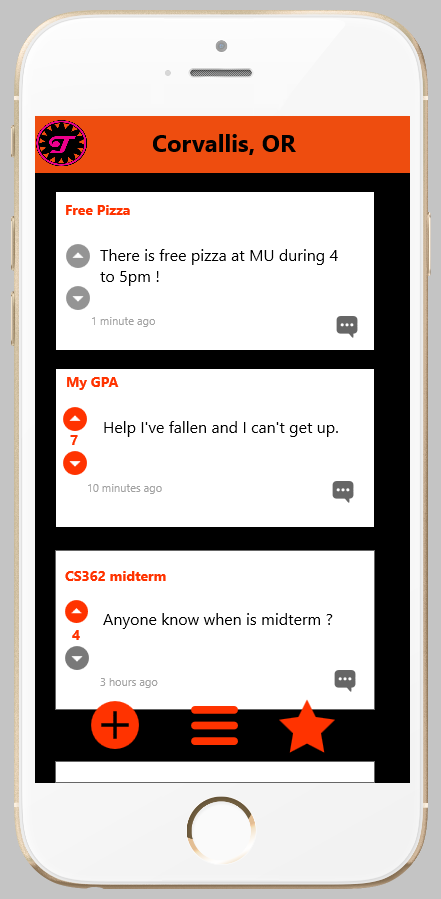
\includegraphics[scale=0.30]{img/ui/post-review}\linebreak
=======
\subsection{Creating a New Post}
Users create a new post with a title and text content. When they press the submit button, a new post element is added to the database, with the attributes of title, text content, submission time, upvote/downvote count, and author as specified by the post class diagram.
\begin{center}
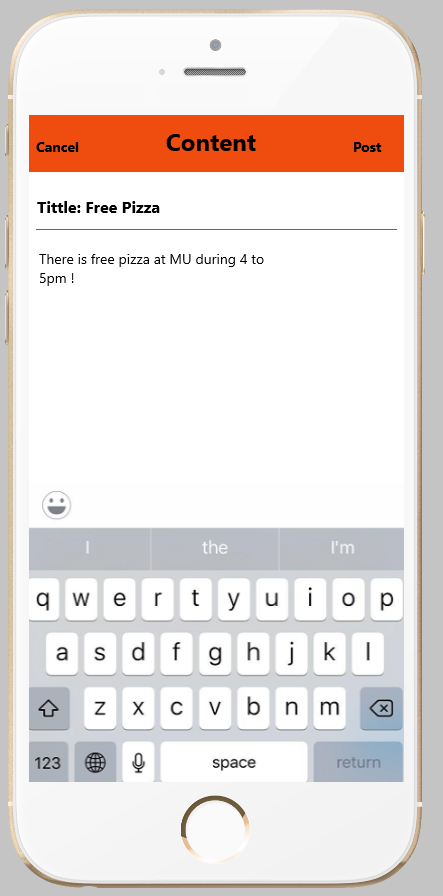
\includegraphics[scale=0.30]{img/ui/post}\linebreak
>>>>>>> 48e1b01a7dc4f75fda74afc716ceda03bda3d7a9
\textbf{Creating a New Post UI}
  \end{center}

\subsection{Auditing New Post}
Post filtering software highlights text that needs to be removed before posting is successful, and prohibits the user from posting until such a condition is met. Examples of prohibited strings include doxxing related strings (phone numbers, addresses), and threat related strings (bomb, kill).
\begin{center}
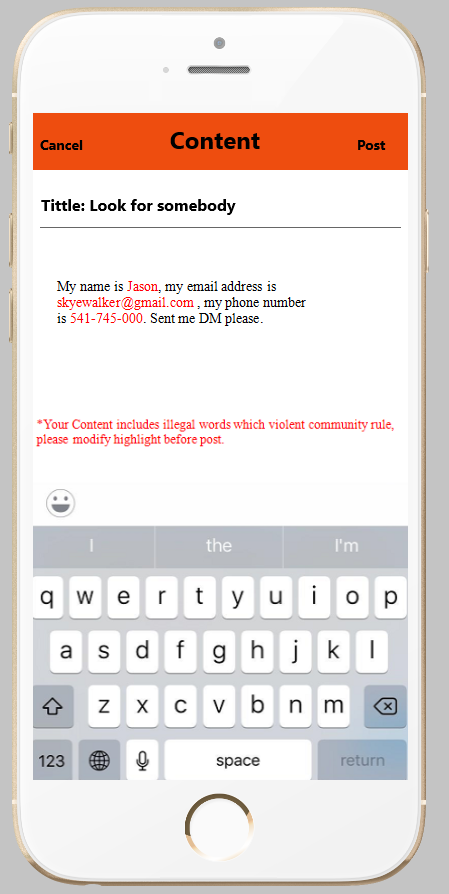
\includegraphics[scale=0.30]{img/ui/bad-post}\linebreak
\textbf{Auditing Result UI}

  \end{center}

\subsection{Viewing Page}
Users view posts on the post viewing page of the app, which is the one that will be loaded when the app starts. Users will view posts sorted by the post sorting function, from which users can select a time range to view posts from, top posts from last 24 hours, week, month, year, or ever. Users will update the posts by pulling down on the top of the app, which will send a request to the server for the updated posts table, which will then be filtered by the post sorting function and displayed to the user in order of time.
\begin{center}
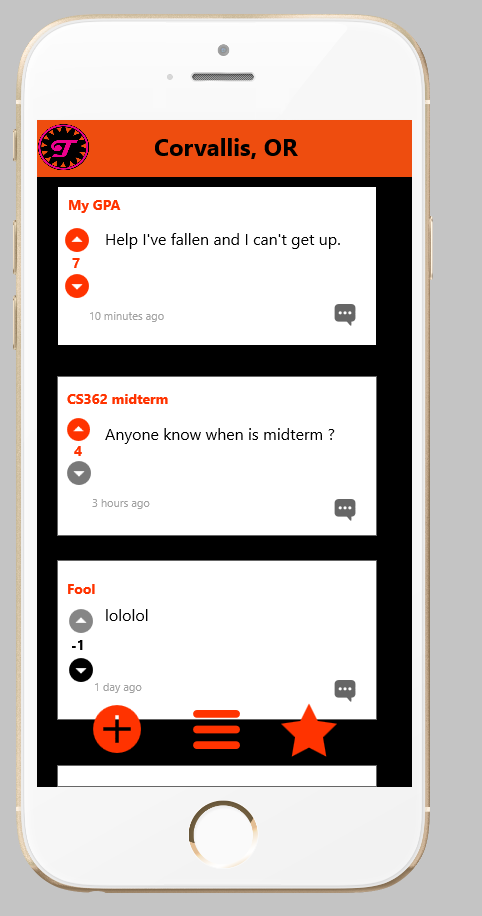
\includegraphics[scale=0.30]{img/ui/view}\linebreak
\textbf{Main Post Page UI}
  \end{center}

\section{Class Diagram}

\section{Sequence Diagram}
\subsection{Creating a New Post}
This is the UML for creating a post. It is designed to be quick and simple with minimal computation.

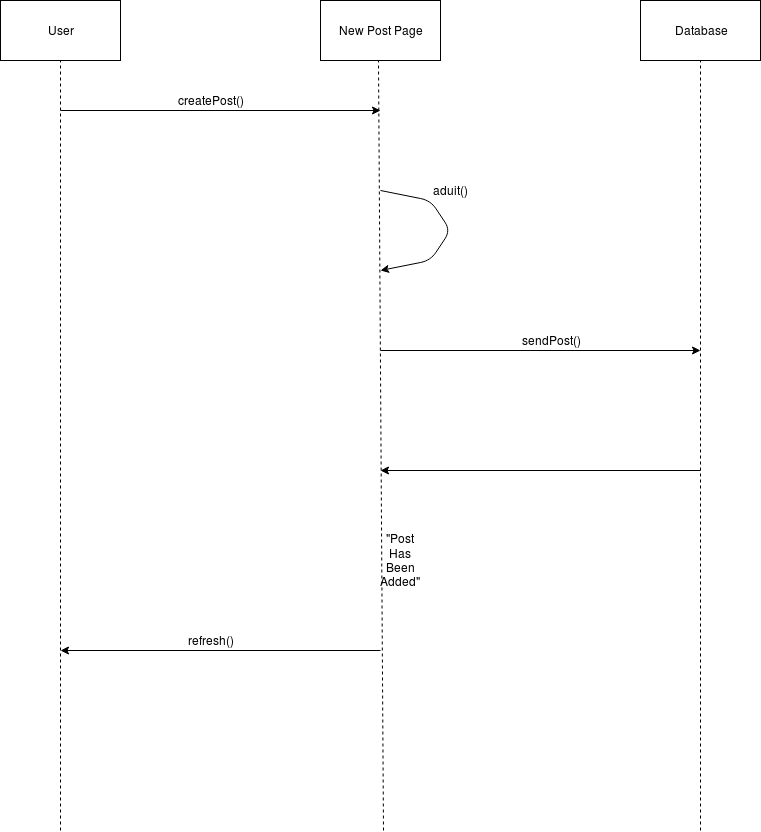
\includegraphics[scale=0.85]{img/uml/createPost}

The user will initiate the new post and be taken to a new post page. They will fill in the requirements. They will hit submit, and their information will be checked to post. If they can post, their submission will be broken from the loop and sent to the database. The information will be updated, the user will be notified, and the page will refresh.
\subsection{Auditing the New Post}
This is the UML for auditing posts. It is made for users to delete their own posts and admins to delete any posts.

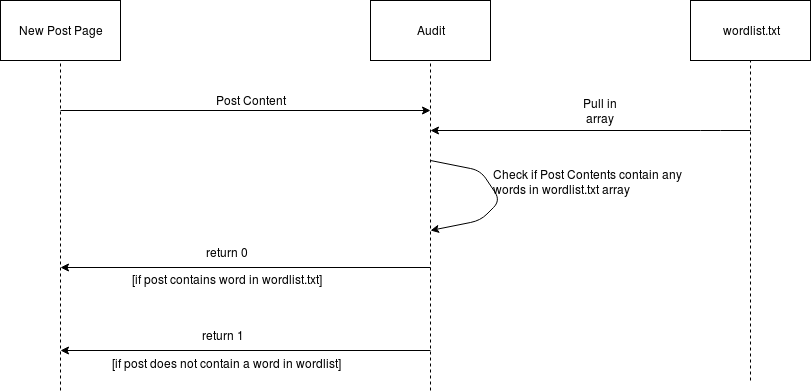
\includegraphics[scale=0.85]{img/uml/audit}

The user will click on a post they want to delete. This will then get checked to see if they are an admin, or if they are the original author. If either condition is met, the post will be deleted from the database. If they fail the if statement, then we know they are a regular user trying to delete someone else’s post.
\subsection{Viewing Post Page}
This its the UML for viewing an entire post. This means that the comments need to be shown. They cannot be upvoted, so the only option a user has is to create a comment.

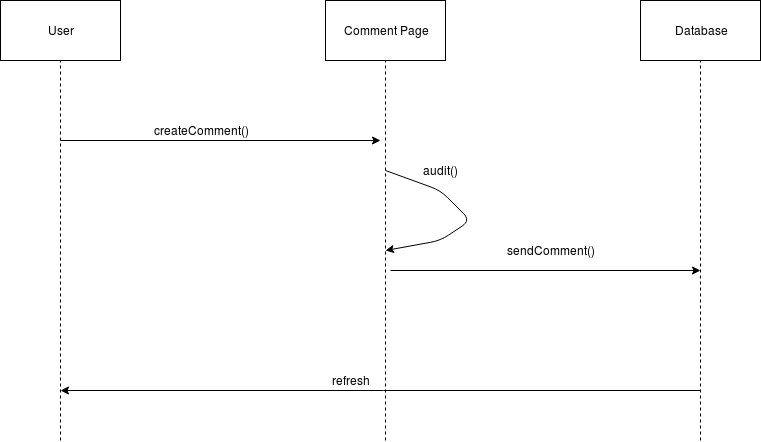
\includegraphics[scale=0.85]{img/uml/createComment}

The user can initiate the comment start, which is taken to the comment page. They will provide the information, and the loop will break once they have met all the conditions. The comment will then be sent to the database, the user will receive a notification, and the page will be refreshed.

\section{Meeting Report}

\subsection{Progress Made This Week}

\subsection{Plans for Next Week}
\subsection{Team Member Contributions}
Github Repo Management/Organization- Aidan Grimshaw, Brendan Byers, Ryan Sisco
User Interface Prototype- Yufei Zeng, Aidan Grimshaw
Class Diagrams- Brendan Byers, Iliana Javier
Sequence Diagrams- Ryan Sisco
Meeting Report- Aidan Grimshaw

\end{document}
